\chapter{基于近场动力学理论的弹塑性本构模型}

\section{近场动力学简介}

\subsection{发展历程}
\label{pdm_history}
作为对固体力学的重新表述或者是一种替代性理论,近场动力学(peridynamics)最开始是由 Silling et al. 在2000年被提出 \mycite{Silling}{2000}。 但不同于传统的经典连续介质力学,近场动力学是一种非局域理论(non-local theory),其假定材料中的物质点不仅仅是受其直接邻域的影响,而是会与在一定半径范围内的所有物质点都发生作用。并且不同于连续介质力学以及几乎所有其他的动力学本构模型,近场动力学理论采用的是一种积分形式的表述,而不是常见的微分形式表达。

最开始的近场动力学理论\mycite{Silling}{2000} 也被称为 bond-based 近场动力学(bond-based peridynamics)。在其表述中,物质中的具有相互作用的物质点对通过约束(bond)相连,相互之间的作用力只与彼此相关,并且具有相同的力大小。因此,基于 bond-based 近场动力学系统实际上可认作是一种质点弹簧系统。 bond-based 近场动力学最大的缺陷是对于各向同性材料,泊松比(Poisson' ratio)被固定为 0.25,这在很大程度上限制了材料的多样性。此外,bond-based 近场动力学不能对体积膨胀和剪切形变进行区分,且无法保证塑性不可压条件,或进一步结合已有的材质模型。所以,bond-based 近场动力学模型虽然在实现上比较简单,但其使用其实是相对受限的。在图形学领域,\mycite{Levine}{2015}第一次使用这一理论在对各向同性的脆性材料进行碎裂仿真。而本文工作,呈现了一个能模拟弹塑性材料和各向异性材料,囊括形变、脆性碎裂、可延展性碎裂等物理现象在内的完整框架。

为解决 bond-based 模型中存在的问题,\mycite{Silling}{2007} 和 \mycite{Emmrich}{2013}进一步对理论进行完善,提出了所谓的 state-based 近场动力学。state-based 近场动力学是一个更为通用的模型,其移除了原有模型关于 0.25 的泊松比限制,并且物质点对之间相互给予的作用力并不一定相同,甚至不一定沿质点之间的连线方向。state-based 模型在材料属性的表达能力上已经与经典连续介质理论具有可比性,因此被工程领域广为采用,其中包括用来做多尺度材质模拟的\mycite{Askari}{2008},\mycite{Silling}{2014a},和用来进行碎裂模拟的\mycite{silling}{2014b},\mycite{Askari}{2006},\mycite{Silling}{2010}。
state-based 近场动力学模型可以进一步分为 Ordinary state-based 和 Non-ordinary state based 模型。其中在Ordinary state based 模型物质点对之间的作用力沿两者直线方向,因此在角动量守恒上自动得到满足,而Non-ordinary state based 作用力可沿其他方向,但仍然需遵守角动量守恒定律。关于三种不同模型的示意,如图\ref{peridynamics_models}所示:

\begin{figure}[htbp!]
  \centering
  \captionsetup{justification=centering}
  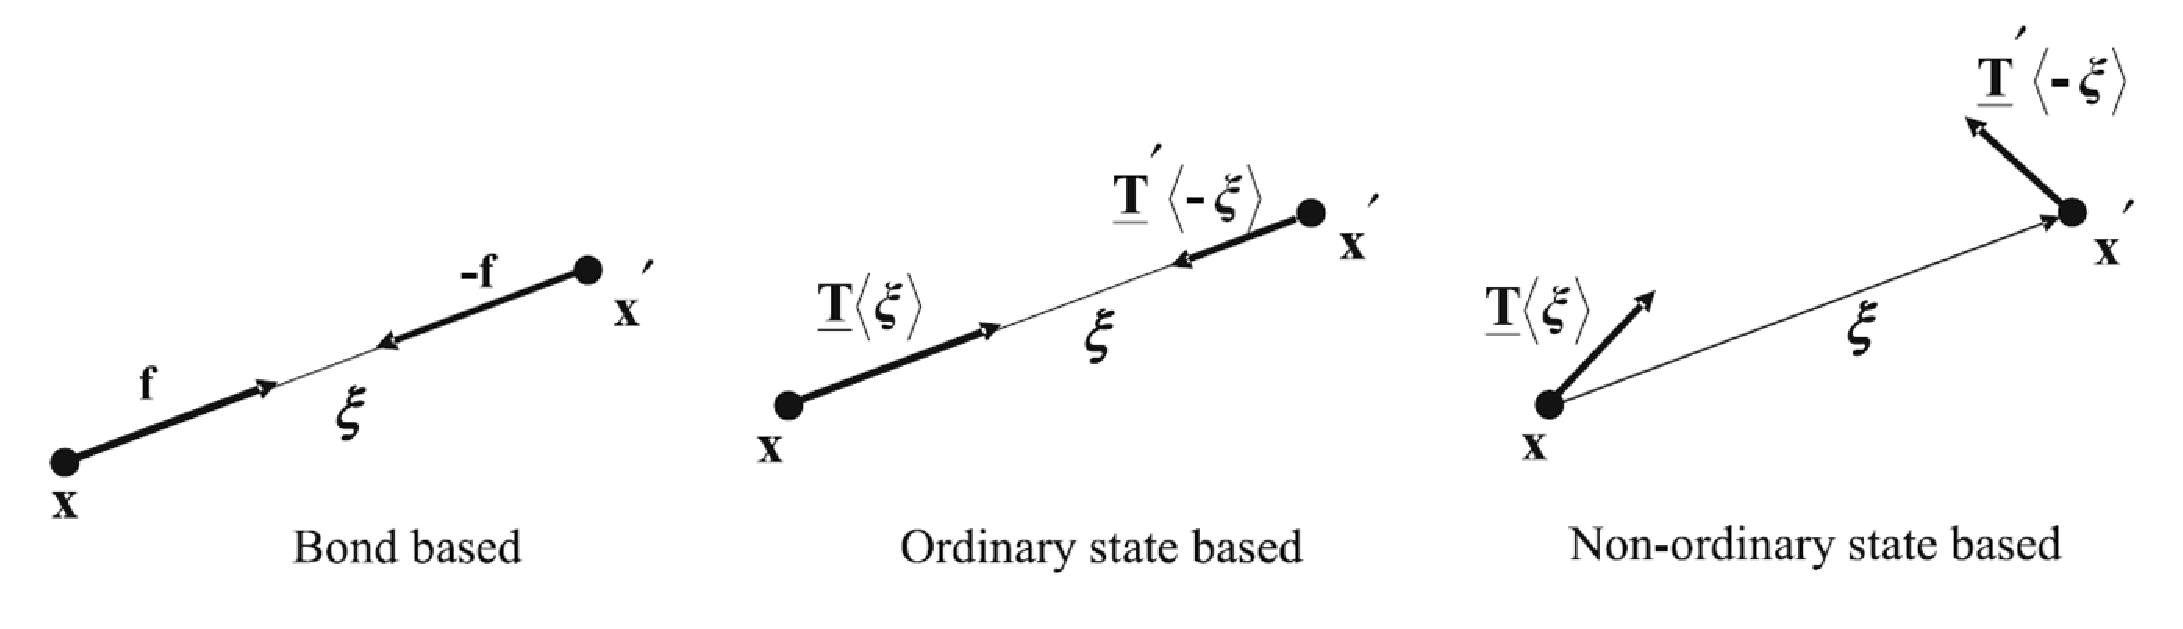
\includegraphics[width=\linewidth]{E:/Thesis-Master/chap/image/peridynamics_models}

  \caption{\label{peridynamics_models}
           bond-based, ordinary state-based, non-ordinary state-based 模型对比示意图。在 bond-based 模型中,粒子之间彼此施加的力相等,且沿两者直线方向,因此本质上是质点弹簧系统。在 ordinary state-based 模型中,力沿两者直线方向,但彼此施加的力不一定相等。在 non-ordinary 模型中,对力的大小和方向并无约束,但需遵守动量和角动量守恒规律。图片取自\mycite{Silling}{2007}。
          }
\end{figure}

虽然近场动力学理论倾向于被认为处理线性弹性材料,但随着近场动力学理论的不断发展,学术界和工业界越来越意识到其理论优越性,其潜力也被不断挖掘,本文工作和其他实践证明其同样可以适用于用于非线性弹性、塑性、粘滞弹性、粘滞塑性材料。限于本文篇幅,在此不可能对近场动力学进行完整的阐述,更详细的介绍请参见\mycite{Madenci}{2014}。 本文工作所用的近场动力学模型基于 ordinary state-based 模型,但对原有理论进行了重新阐述以及修改,以适应图形学领域应用的特点。

\subsection{基本特征和形式}
\label{pdm_basic_feature}
在上节中已经提及,相对于其他动力学模型,近场动力学的两大基本特点分别是非局域性以及积分形式的表述。

关于粒子之间作用的局域性问题,存在两种截然不同的理论。以经典连续介质力学为代表的局域性理论,认为粒子在微观上只和其直接邻域发生作用,而和其他粒子无关。这一假设在很大程度上对材质进行了简化,却又基本上描述了材料的动力学行为,因而在工程领域以及图形学领域应用极多。局域性理论的另一个极端则是分子动力学,其认为每一个粒子和其他粒子都能彼此发生作用,而不仅限于其直接邻居。分子动力学在基础物理领域的仿真应用较大,但在倾向于研究宏观运动行为的图形学领域则应用较少。从局域性的观点来看,近场动力学恰好位于两种理论之间,其假定材质中的物质点会和有限半径范围内的邻域发生作用,因此可认作是连接两种理论的桥梁。如图\ref{peridynamics_comparison}所示:

\begin{figure}[htbp!]
  \centering
  \captionsetup{justification=centering}
  \includegraphics[width=\linewidth]{E:/Thesis-Master/chap/image/peridynamics_comparison}

  \caption{\label{peridynamics_comparison}
           不同动力学模型的作用域大小对比。左边为局域性理论,粒子只和直接邻域发生相互作用。右边为分子动力学理论,可认定作用半径无限大。而近场动力学位于两者之间,受邻域半径 $\delta$ 范围内的粒子影响。
          }
\end{figure}

对于近场动力学模型,可以根据图\ref{peridynamics_comparison}中图作更为细致的形式化表述。具体而言,材质中的任何一个物质粒子 $\mathbf{x}$ 将会和其周边半径为 $\delta$ 内的粒子发生相互作用,这一半径 $\delta$ 被定义为\textbf{邻域半径}(horizon),而位于邻域半径 $\delta$ 之内的粒子被定义\textbf{邻域}(family),$H_\mathbf{x}$。对于连续性的材料,在离散化之前,邻域范围内的粒子数量可认定是无穷的。从用粒子来表示物体的观点来看,近场动力学的基本思想和其他无网格方法\textcolor{blue}{(M\"{u}ller et al.)\parencite{Muller2003}\parencite{Muller2003}}并无大差异,最大的区别在作用半径 $\delta$ 的定义,这也是近场动力学理论被认定为非局域性理论的原来。 \mycite{Silling}{2003}证明,当 $\delta$ 趋向于0 时,近场动力学模型将会退化为经典的连续介质力学。而当 $\delta$ 区域无穷大时,则会成为连续形式的分子动力学理论。

在近场动力学之前,几乎所有的动力学模型都采用的是微分形式的本构方程(governing function)。最为典型的就是在连续介质力学理论中,本构方程一般使用如下形式,

\begin{equation}
\label{fem_governing_function}
\rho\ddot{\mathbf{u}}(\mathbf{x}) = \nabla\cdot\delta(\mathbf{x})+\mathbf{b}(\mathbf{x})
\end{equation}

其中$\rho$表示粒子的质量密度。$\ddot{\mathbf{u}}$为向量,表示粒子的位移。$\mathbf{b}$表示粒子所受外力,一般包括重力或者由碰撞导致的外力等。类似的符号表示将同样应用于后续近场动力学的本构方程,后面将不再赘述。在方程\ref{fem_governing_function}中,另一个最为关键的物理量是$\nabla\cdot\delta$,即是二阶应力张量$\delta$的散度微分,表示单位体积物理所受的力(力密度)。如前面章节\ref{constitutive_model} 所述, $\delta$的计算尤为关键,其包含物体所有的本构信息。需要尤其注意的是,$\nabla\cdot\delta$ 是关于空间位置的偏微分,而空间微分在不连续之处并不能很好定义,在物体边界以及碎裂发生之处,空间微分很容易导致奇异值问题。因此在基于连续介质力学的离散框架(FEM)以及相关工作中,往往需要额外的工作来特殊对待碎裂问题,例如textcolor{blue}{(O'Brien et al. 1999)\parencite{OBrien1999}},\textcolor{blue}{(O'Brien et al. 2002)\parencite{OBrien2002}}中的 remeshing 操作。事实上,这一问题并不仅仅存在于有网格方法,\mycite{Madenci}{2014}指出,几乎所有的无网格方法使用的都是微分形式的本构方程,因而都不能避免此问题。

不同于以往方法,近场动力学使用的是积分形式的动力学表述,这也是其另一大特征。由于是积分形式,近场动力学的本构方程在不连续处将仍然保持良好定义,并且材质的损伤本身就是模型的一部分。这一优势使得近场动力学非常适合处理不连续问题,尤为是碎裂现象。具体而言,近场动力学中关于物质粒子 $\mathbf{x}$的本构方程可以写为

\begin{equation}
\rho\ddot{\mathbf{u}}(\mathbf{x}) = \int_{H_\mathbf{x}}[\mathbf{T}\langle\mathbf{x}',\mathbf{x}\rangle - \mathbf{T}\langle\mathbf{x},\mathbf{x}'\rangle]dH+\mathbf{b}(\mathbf{x}),
\label{pdm_governing_function}
\end{equation}

其中$\rho, \mathbf{u}, \mathbf{b}$ 的含义同\ref{fem_governing_function}一致。$\mathbf{x}'$ 表示属于 $\mathbf{x}$ 的邻域 $H_\mathbf{x}$ 另外一个物质粒子。$\mathbf{T}\langle\mathbf{x}',\mathbf{x}\rangle$ 和 $\mathbf{T}\langle\mathbf{x},\mathbf{x}'\rangle$ 是两个关键变量,其包含了材质的本构信息。$\mathbf{T}\langle\mathbf{x}',\mathbf{x}\rangle$ 表示粒子 $\mathbf{x}'$ 施加给粒子 $\mathbf{x}$ 的内力,而$\mathbf{T}\langle\mathbf{x},\mathbf{x}'\rangle$ 则相反,表示粒子 $\mathbf{x}$ 施加给粒子 $\mathbf{x}'$ 的内力。注意如章节\ref{pdm_history}所述,这两个变量并不一定相同,但必须同时出现在本构方程中以遵循牛顿第三定律,这一策略类似于 SPH 方法\textcolor{blue}{(M\"{u}ller et al. 2003)\parencite{Muller2003}}。尖括号$\langle\cdot\rangle$ 符号表示关于 $H_\mathbf{x}$的函数,其在\mycite{Silling}{2007}中被定义为\textbf{状态}(state)。需要尤其注意的是本构方程中的积分符号 $\int_{H_\mathbf{x}}$,这是近场动力学模型区别其他理论最根本上的不同。可以看出,整个方程是基于粒子的位移$\mathbf{u}$,而不是基于位移的空间微分的,因此也使得对于不连续问题的处理更加方便以及稳定。在粒子离散框架下,关于邻域 $H_\mathbf{x}$ 的连续积分可以进一步用粒子的累加和来表示,即,

\begin{equation}
\rho\ddot{\mathbf{u}}(\mathbf{x}) = \sum_{\mathbf{x}'\in H_\mathbf{x}}[\mathbf{T}\langle\mathbf{x}',\mathbf{x}\rangle - \mathbf{T}\langle\mathbf{x},\mathbf{x}'\rangle]V_{\mathbf{x}'}+\mathbf{b}(\mathbf{x}),
\label{pdm_governing_function_discrete}
\end{equation}
其中 $V_{\mathbf{x}'}$ 表示粒子 $\mathbf{x}'$ 的体积,其值取决于粒子的分布。

\section{模型推导}
在章节\ref{pdm_basic_feature}中,公式\ref{pdm_governing_function_discrete}描述了近场动力学的基本形式和本构方程。但更为关键的是两个重要变量$\mathbf{T}\langle\mathbf{x}',\mathbf{x}\rangle$ 和 $\mathbf{T}\langle\mathbf{x},\mathbf{x}'\rangle$,其蕴含了材质的本构信息,需要以更为形式化的方式来进行表述。$\mathbf{T}\langle\cdot\rangle$ 的具体形式需要通过发掘材质属性,以及物理规律推导来获得,较为合理的方式便是建立在已有的经典连续介质力学基础之上,然后将两个理论进行等效。但由于连续介质力学是局域性的理论,因此我们首先需要对近场动力学作局域性假设。

\subsection{局域性假设}
在极限情况下,亦即当$\delta$ 趋于0时,可认为物质粒子 $\mathbf{x}$ 仅和其直接邻居发生相互作用。如图所示,标记为 $k$ 的粒子只和周围六个粒子 $(k-l)$,$(k+l)$,$(k-m)$,$(k+m)$,$(k-n)$,和$(k+n)$ 存在力作用。这和经典连续介质力学一致,参见\mycite{Bonet}{2008}。

\begin{figure}[htbp!]
  \centering
  \captionsetup{justification=centering}
  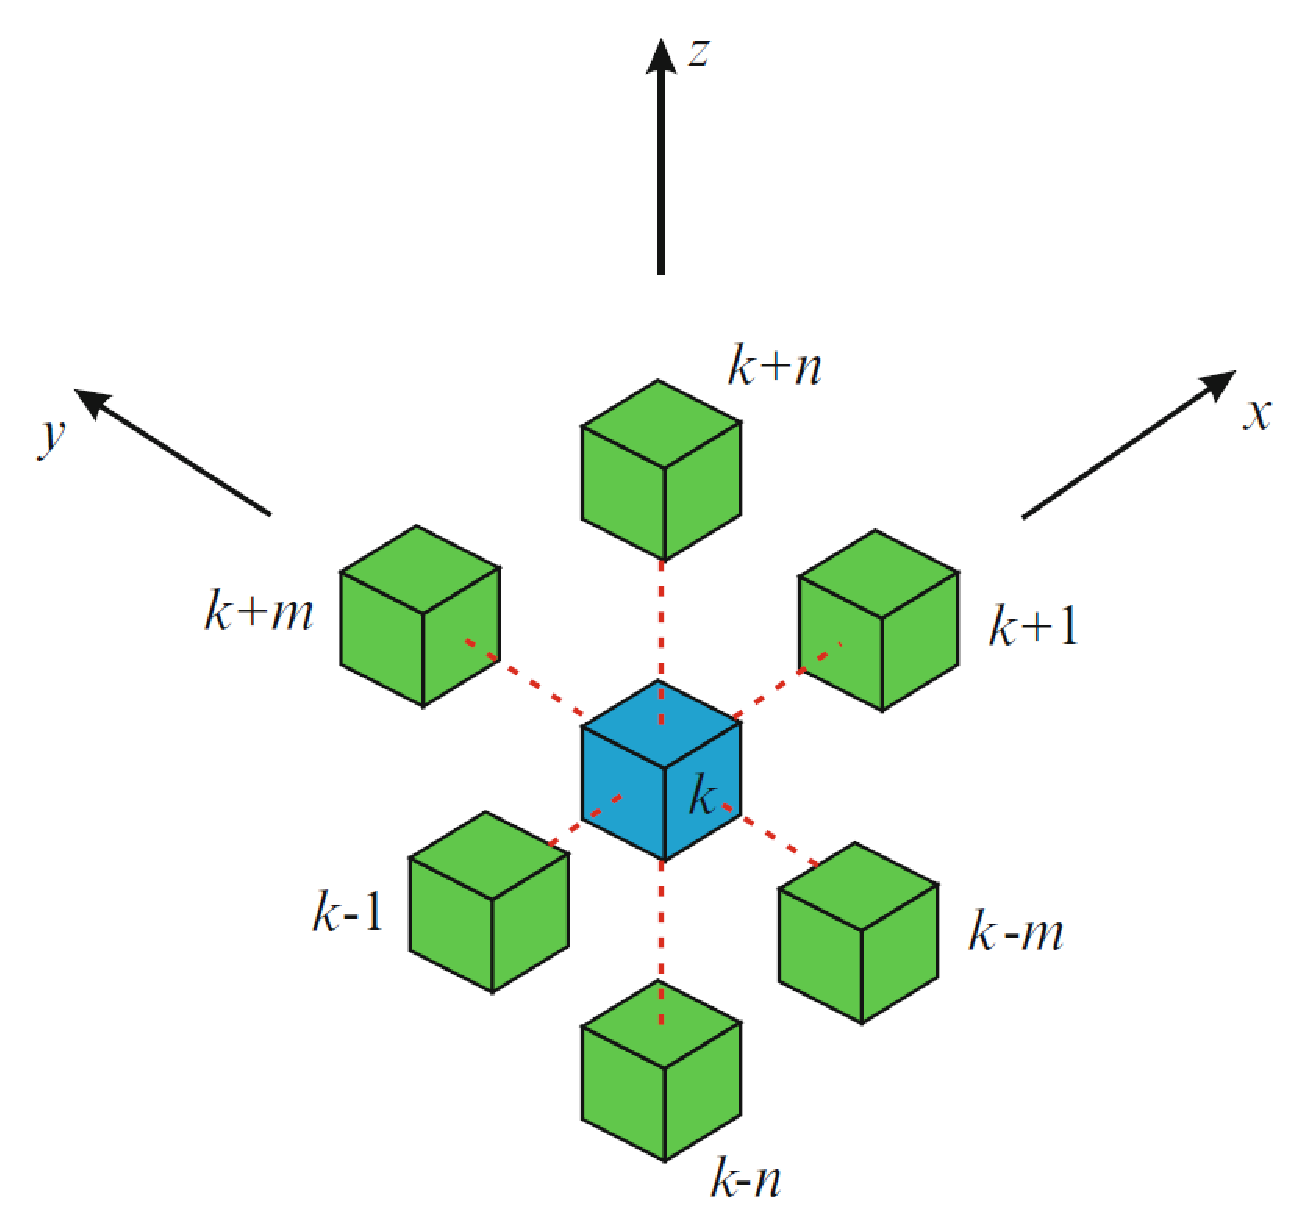
\includegraphics[width=0.5\linewidth]{E:/Thesis-Master/chap/image/pdm_local}

  \caption{\label{pdm_local}
           局域性假设下的近场动力学。物质粒子 $\mathbf{x}$ 仅仅和$(k-l)$,$(k+l)$,$(k-m)$,$(k+m)$,$(k-n)$,和 $(k+n)$ 周围六个粒子相互作用。图片取自\mycite{Madenci}{2014}。
          }
\end{figure}

在局域性假设下,针对粒子 $k$,公式\ref{pdm_governing_function_discrete}则可以写成如下形式,
\begin{equation}
\rho_{(k)}\ddot{\mb{u}}_{(k)}
= \sum_{j=k-l,k+l,k-m,k+m,k-n,k+n}(\mb{t}_{(k)(j)}-\mb{t}_{(j)(k)})V_{(j)} + \mb{b}_{(k)}
\label{pdm_local_governing_function}
\end{equation}
这里 $\mb{t}_{(k)(j)}$ 表示物质粒子 $j$ 施加给物质粒子 $k$的内力密度,而$\mb{t}_{(j)(k)}$ 表示物质粒子 $k$ 施加给物质粒子 $j$的内力密度。根据中心差分公式,经典连续介质力学中的本构方程(即公式\ref{fem_governing_function})可以写成分量形式,以 $x$ 分量为例,有

\begin{equation}
\begin{aligned}
\rho_{(k)}\ddot{\mb{u}}_{x(k)} &= \quad \frac{1}{2}\frac{\sigma_{xx(k)} - \sigma_{xx(k-l)}}{\Delta x} + \frac{1}{2}\frac{\sigma_{xx(k+l)} - \sigma_{xx(k)}}{\Delta x}\\
                              &\quad+  \frac{1}{2}\frac{\sigma_{xy(k)} - \sigma_{xy(k-m)}}{\Delta y} + \frac{1}{2}\frac{\sigma_{xy(k+m)} - \sigma_{xy(k)}}{\Delta y}\\
                              &\quad+  \frac{1}{2}\frac{\sigma_{zx(k)} - \sigma_{zx(k-n)}}{\Delta z} + \frac{1}{2}\frac{\sigma_{xz(k+n)} - \sigma_{xz(k)}}{\Delta z}\\
                              &\quad + \mb{b}_{x(k)}
\label{fem_local_governing_function}
\end{aligned}
\end{equation}
在上式中,每一项都仅仅和物质粒子 $k$ 以及直接邻居相关。我们可以将公式\ref{pdm_local_governing_function}写成类似的形式,即

\begin{equation}
\begin{aligned}
\rho_{(k)}\ddot{\mb{u}}_{(k)} &= \quad (\mb{t}_{(k)(k-l)} - \mb{t}_{(k-l)(k)})V_{(k-l)} + (\mb{t}_{(k)(k+l)} - \mb{t}_{(k+l)(k)})V_{(k+l)}\\
                             &\quad + (\mb{t}_{(k)(k-m)} - \mb{t}_{(k-m)(k)})V_{(k-m)} + (\mb{t}_{(k)(k+m)} - \mb{t}_{(k+m)(k)})V_{(k+m)}\\
                             &\quad + (\mb{t}_{(k)(k-n)} - \mb{t}_{(k-n)(k)})V_{(k-n)} + (\mb{t}_{(k)(k+n)} - \mb{t}_{(k+n)(k)})V_{(k+n)}\\
                             &\quad  + \mb{b}_{(k)}
\label{pdm_local_governing_function_2}
\end{aligned}
\end{equation}

通过比较方程 \ref{fem_local_governing_function} 和方程 \ref{pdm_local_governing_function_2},可以得到关于柯西应力和内力密度的关系,即

\begin{equation}
\sigma_{\alpha\beta(k)} = 2t_{\beta(k)(q_\alpha)}\Delta\alpha V_{(q_\alpha)}\qquad \mathrm{with } \quad q_x=(k+l),q_y=(k+m),q_z=(k+n)
\label{eq:7}
\end{equation}
\begin{equation}
\sigma_{\alpha\beta(k)} = -2t_{\beta(k)(q_\alpha)}\Delta\alpha V_{(q_\alpha)}\qquad \mathrm{with } \quad q_x=(k-l),q_y=(k-m),q_z=(k-n),
\label{eq:8}
\end{equation}

其中$\alpha,\beta=x,y,z$。对于正压力(normal stress),我们有

\begin{equation}
\sigma_{\alpha\alpha} = 2 \mb{t}_{(k)(q_\alpha)}\cdot(\mb{x}_{(q_\alpha)}-\mb{x}_{k})V_{(q_\alpha)}.
\label{eq:9}
\end{equation}

还可以进一步得到

\begin{equation}
\begin{aligned}
\sum_{\beta=x,y,z}\sigma_{\alpha\beta(k)}^2 &= \sum_{\beta=x,y,z}4t_{\beta(k)(q_\alpha)}^2(\Delta\alpha)^2 V_{(q_\alpha)}^2 \\
                                            &= 4(\mb{t}_{(k)(q_\alpha)}|\mb{x}_{(q_\alpha)}-\mb{x}_{k}|V_{(q_\alpha)})
                                                 \cdot
                                                (\mb{t}_{(k)(q_\alpha)}|\mb{x}_{(q_\alpha)}-\mb{x}_{k}|V_{(q_\alpha)}).
\end{aligned}
\label{eq:10}
\end{equation}

这一关系式将会在后续章节使用到。

\subsection{应变能量密度和内力密度}
在连续介质力学中,超弹性本构模型一般采用应变能量密度来进行表示(strain energy density),因此有必要建立应变能量密度和近场动力学中内力密度的关系。根据哈密顿力学理论,以及\mycite{Silling}{2007}关于ordinary state-based模型的定义,近场动力学中的内力密度可定义如下

\begin{equation}
\mb{t}_{(k)(j)}=\frac{1}{V_{(j)}}\frac{\partial W_{(k)}}{\partial (|\mb{y}_{(j)}-\mb{y}_{(k)}|)}\frac{\mb{y}_{(j)}-\mb{y}_{(k)}}{|\mb{y}_{(j)}-\mb{y}_{(k)}|},
\label{eq:11}
\end{equation}

其中 $W_{(k)}$ 表示物质粒子 $k$ 的应变能量密度。注意,力密度向量是和物质粒子之间的连线方向重合的,因而直接满足角动量守恒定律。上式可简写为
\begin{equation}
\mb{t}_{(k)(j)} = \frac{1}{2}A\frac{\mb{y}_{(j)}-\mb{y}_{(k)}}{|\mb{y}_{(j)}-\mb{y}_{(k)|}}
\label{eq:12}
\end{equation}
及
\begin{equation}
\mb{t}_{(j)(k)} = -\frac{1}{2}B\frac{\mb{y}_{(j)}-\mb{y}_{(k)}}{|\mb{y}_{(j)}-\mb{y}_{(k)|}},
\label{eq:13}
\end{equation}

其中$A$ 和 $B$ 是辅助变量,取决于物质的材质参数,形变,以及邻域半径 $\delta$。

\subsection{超弹性模型通用推导框架}
给定连续介质力学中某一超弹性模型的应变能量表示,我们可以通过遵循相同的步骤来推得近场动力学中内力密度的具体形式。而一旦获得内力密度的显式形式,便可以进一步推导得到在近场动力学理论下的本构方程,从而进行后续的仿真工作。

对于一般模型的超弹性材质的推导步骤总结如下:
\begin{enumerate}
  \item 使用内力密度 $\mathbf{t}$ 来表示应变能量密度 $W$。通常而言,在连续介质力学中,应变能量密度通常通过应力张量 $\delta$ 来进行表示,或者可以方便地转换为此种形式。然后通过应力张量 $\delta$ 和内力密度 $\mathbf{t}$的关系(即\ref{eq:7} ~ \ref{eq:10}),我们就可以直接建立应变能量密度 $W$ 和$\mathbf{t}$之间的联系。
  \item 将 $\mathbf{t}$ (方程 \ref{eq:12}和\ref{eq:13})代入到能量密度 $W$ 的表达式,并根据式 \ref{eq:11} 执行微分操作,获得力密度$\mathbf{t}$的具体形式。
  \item 在多种不同的简单受力情况下,通过比较连续介质力学中的应变能量密度以及近场动力学中对应的部分来确定相应的材质辅助参数。选择的受力情况一般应尽量简单,并且是可以在连续介质力学中进行解析计算的。最后可以令两者能量相等,获得近场动力学中的材质参数。
\end{enumerate}

本文下面将通过线性弹性模型的推导来具体展示这一流程,这也是本文工作所用模型。根据上述步骤,还可以推得其他超弹性模型在近场动力学理论中的表示,例如 FEM 中常用的不可压 Neo-Hookean 材质模型 \mycite{Bang}{2016}。

\subsection{线性弹性模型推导}
\subsubsection{步骤1:使用内力密度表达应力能量密度}
对于连续介质力学中的各向同性线性弹性材料,对于物质粒子 $k$,应变能量密度 $W(k)$ 的具体形式可写为

\begin{equation}
W_{(k)} = \frac{\kappa}{2}\theta_{(k)}^2+\left[\frac{1}{4\mu}(\sigma_{xx(k)}^2+\sigma_{yy(k)}^2+\sigma_{zz(k)}^2)
                                         +\frac{1}{2\mu}(\sigma_{xy(k)}^2+\sigma_{xz(k)}^2+\sigma_{yz(k)}^2)
                                         -\frac{3\kappa^2}{4\mu}\theta_{(k)}^2
                                    \right],
\label{eq:14}
\end{equation}

其中 $\kappa$ 和 $\mu$ 与前述章节一致,分别为体积模量和剪切模量。上式右边第一项衡量的是材质的各向均匀膨胀能量,而第二项衡量的是剪切能量。膨胀度 $\theta_{(k)}$(dilatation)被定义为

\begin{equation}
\theta_{(k)} = \epsilon_{xx(k)}+\epsilon_{yy(k)}+\epsilon_{zz(k)} = \frac{\sigma_{xx(k)}+\sigma_{yy(k)}+\sigma_{zz(k)}}{3\kappa}.
\label{eq:15}
\end{equation}

对式\ref{eq:14}稍微进行重整,则可以得到

\begin{equation}
\begin{aligned}
W_{(k)} =& \frac{\kappa}{2}\theta_{(k)}^2 -\frac{3\kappa^2}{4\mu}\theta_{(k)}^2 \\
         &+\frac{1}{8\mu}\left[(\sigma_{xx(k)}^2+\sigma_{xy(k)}^2+\sigma_{xz(k)}^2) + (\sigma_{xx(k)}^2+\sigma_{xy(k)}^2+\sigma_{xz(k)}^2)\right]\\
         &+\frac{1}{8\mu}\left[(\sigma_{yx(k)}^2+\sigma_{yy(k)}^2+\sigma_{yz(k)}^2) + (\sigma_{yx(k)}^2+\sigma_{yy(k)}^2+\sigma_{yz(k)}^2)\right]\\
         &+\frac{1}{8\mu}\left[(\sigma_{zx(k)}^2+\sigma_{zy(k)}^2+\sigma_{zz(k)}^2) + (\sigma_{zx(k)}^2+\sigma_{zy(k)}^2+\sigma_{zz(k)}^2)\right],
\end{aligned}
\label{eq:16}
\end{equation}

在上式中,关于应力张量的每一项被分别对应于粒子 $k$ 的六个直接邻居$(k-l)$,$(k+l)$,$(k-m)$,$(k+m)$,$(k-n)$ 和 $(k+n)$。使用式 \ref{eq:10} 建立的关系,可得

\begin{equation}
\begin{aligned}
W_{(k)} =& (\frac{\kappa}{2} -\frac{3\kappa^2}{4\mu})\theta_{(k)}^2 \\
         &+\frac{1}{2\mu}\sum_{\substack {j=k-l,k+l,\\ \quad k-m,k+m,\\ \quad k-n,k+n}}(\mb{t}_{(k)(j)}|\mb{x}_{(j)}-\mb{x}_{(k)}|V_{(j)})\cdot(\mb{t}_{(k)(j)}|\mb{x}_{(j)}-\mb{x}_{(k)}|V_{(j)}).
\end{aligned}
\label{eq:17}
\end{equation}

同样可以将膨胀度 $\theta_{(k)}$ 写成分别对应六个邻居粒子的形式

\begin{equation}
\begin{aligned}
\theta_{(k)} =& \frac{\sigma_{xx(k)}+\sigma_{yy(k)}+\sigma_{zz(k)}}{3\kappa}\\
        =& \frac{1}{3\kappa}(\frac{1}{2}\sigma_{xx(k)}+\frac{1}{2}\sigma_{yy(k)}+\frac{1}{2}\sigma_{zz(k)}
         + \frac{1}{2}\sigma_{xx(k)}+\frac{1}{2}\sigma_{yy(k)}+\frac{1}{2}\sigma_{zz(k)}).
\end{aligned}
\label{eq:18}
\end{equation}

将式 \ref{eq:9} 代入上述方程, 则可以获得$\theta_{(k)}$关于$\mb{t}_{(k)}$的具体形式

\begin{equation}
\theta_{(k)} = \frac{1}{3\kappa}\left(\sum_{\substack {j=k-l,k+l,\\ \quad k-m,k+m,\\ \quad k-n,k+n}}(\mb{t}_{(k)(j)}\cdot(\mb{x}_{(j)}-\mb{x}_{(k)})V_{(j)})\right).
\label{eq:19}
\end{equation}

结合式 \ref{eq:17} 和式 \ref{eq:19},便可以通过内力密度$\mb{t}_{(k)(j)}$来具体表示能量$W_{(k)}$。

\subsubsection{步骤2:获得力密度具体形式}
对于各向同性的线性弹性材料,物质粒子间的内力为线性关系,也就是其大小和 bond 之间的伸长度呈正比例关系。因此,内力密度$\mb{t}_{(k)(j)}$可以写为更为具体的形式

\begin{equation}
\mb{t}_{(k)(j)} = \frac{1}{2}cs_{(k)(j)}\frac{\mb{y}_{(j)} - \mb{y}_{(k)}}{|\mb{y}_{(j)} - \mb{y}_{(k)}|},
\label{eq:20}
\end{equation}
其中
\begin{equation}
s_{(k)(j)} = \frac{|\mb{y}_{(j)} - \mb{y}_{(k)}| - |\mb{x}_{(j)} - \mb{x}_{(k)}|}{|\mb{x}_{(j)} - \mb{x}_{(k)}|}
\label{eq:21}
\end{equation}
为物质粒子间的伸长比例, $c$ 类似于质点弹簧系统中弹簧的弹性系数。

将式\ref{eq:20} 代入到式 \ref{eq:17} 和 \ref{eq:19},可得
\begin{equation}
\begin{aligned}
W_{(k)} =& (\frac{\kappa}{2} -\frac{3\kappa^2}{4\mu})\theta_{(k)}^2 \\
         &+\frac{c^2}{8\mu}\sum_{\substack {j=k-l,k+l,\\ \quad k-m,k+m,\\ \quad k-n,k+n}}(s_{(k)(j)}|\mb{x}_{(j)}-\mb{x}_{(k)}|V_{(j)})\cdot(s_{(k)(j)}|\mb{x}_{(j)}-\mb{x}_{(k)}|V_{(j)})
\end{aligned}
\label{eq:22}
\end{equation}
\begin{equation}
\theta_{(k)} = \frac{c}{6\kappa}\left(\sum_{\substack {j=k-l,k+l,\\ \quad k-m,k+m,\\ \quad k-n,k+n}}\left(s_{(k)(j)}\frac{\mb{y}_{(j)} - \mb{y}_{(k)}}{|\mb{y}_{(j)} - \mb{y}_{(k)}|}\cdot(\mb{x}_{(j)}-\mb{x}_{(k)})V_{(j)}\right)\right).
\label{eq:23}
\end{equation}

通过替换其中的常数系数,上述两式可以写为更一般化的形式

\begin{equation}
W_{(k)} = a\theta_{(k)}^2 + \sum_{\substack {j=k-l,k+l,\\ \quad k-m,k+m,\\ \quad k-n,k+n}}b(s_{(k)(j)}|\mb{x}_{(j)}-\mb{x}_{(k)}|V_{(j)})\cdot(s_{(k)(j)}|\mb{x}_{(j)}-\mb{x}_{(k)}|V_{(j)})
\label{eq:24}
\end{equation}
\begin{equation}
\theta_{(k)} = d\left(\sum_{\substack {j=k-l,k+l,\\ \quad k-m,k+m,\\ \quad k-n,k+n}}\left(s_{(k)(j)}\frac{\mb{y}_{(j)} - \mb{y}_{(k)}}{|\mb{y}_{(j)} - \mb{y}_{(k)}|}\cdot(\mb{x}_{(j)}-\mb{x}_{(k)})V_{(j)}\right)\right).
\label{eq:25}
\end{equation}
其中$a$, $b$ 和 $d$ 为未决的动力学参数。

到目前为止,本文讨论的仍然在局域性假设下的近场动力学模型推导。可以通过直接扩充其作用半径,将这一模型应用到非局域的情形下,即
\begin{equation}
W_{(k)} = a\theta_{(k)}^2 + b\sum_{j=1}^{N}\omega_{(k)(j)}(s_{(k)(j)}|\mb{x}_{(j)}-\mb{x}_{(k)}|V_{(j)})\cdot(s_{(k)(j)}|\mb{x}_{(j)}-\mb{x}_{(k)}|V_{(j)})
\label{eq:26}
\end{equation}
\begin{equation}
\theta_{(k)} = d\sum_{j=1}^{N}\omega_{(k)(j)}s_{(k)(j)}\frac{\mb{y}_{(j)} - \mb{y}_{(k)}}{|\mb{y}_{(j)} - \mb{y}_{(k)}|}\cdot(\mb{x}_{(j)}-\mb{x}_{(k)})V_{(j)}.
\label{eq:27}
\end{equation}

其中$\sum_{\substack {j=k-l,k+l,\\ \quad k-m,k+m,\\ \quad k-n,k+n}}$ 被替换为 $\sum_{j=1}^{N}$,$N$ 表示在粒子 $k$ 邻域 $H_{\mb{x}}$ 中和其进行相互作用的粒子数量。此外,$\omega_{(k)(j)}$ 为权重函数,用来控制粒子 $k$ 对邻域内粒子的影响程度,定义为

\begin{equation}
\omega_{(k)(j)} = \frac{\delta}{|\mb{x}_{(j)}-\mb{x}_{(k)}|}.
\label{eq:28}
\end{equation}

注意 $\omega_{(k)(j)}$ 与方向无关,也就是模型是各向同性的。显而易见,当邻域内粒子离中心粒子 $k$ 越近时,则权重更大。利用式 \ref{eq:11} 所述内力密度定义,即可以获得 $\mb{t}_{(k)(j)}$ 的最终形式。

\begin{equation}
\mb{t}_{(k)(j)} = \frac{1}{2}A\frac{\mb{y}_{(j)} - \mb{y}_{(k)}}{|\mb{y}_{(j)} - \mb{y}_{(k)}|}
\label{eq:29}
\end{equation}
其中
\begin{equation}
A = 4\omega_{(k)(j)}\left\{ad\frac{\mb{y}_{(j)} - \mb{y}_{(k)}}{|\mb{y}_{(j)} - \mb{y}_{(k)}|}\cdot\frac{\mb{x}_{(j)} - \mb{x}_{(k)}}{|\mb{x}_{(j)} - \mb{x}_{(k)}|}\theta_{(k)}
   +b\left(|\mb{y}_{(j)} - \mb{y}_{(k)}| - |\mb{x}_{(j)} - \mb{x}_{(k)}|\right) \right\}.
\label{eq:30}
\end{equation}

\subsubsection{步骤3:确定近场动力学参数}

在上节中,我们已经获取关于内力密度的表述式(\ref{eq:30}),仍其中存在三个未知的动力学参数($a, b, d$)需要确定。本节则通过两种简单的形变受力情况(各向均匀膨胀和简单剪切)来确认这些参数。\\

\noindent{\textbf{Case 1: 各向均匀膨胀}}

各向均匀膨胀可以通过对材质各方向应用一个统一的应变 $\zeta$ 来实现,如图 \ref{pdm_isotropic_expansion} 所示。

\begin{figure}[htbp!]
  \centering
  \captionsetup{justification=centering}
  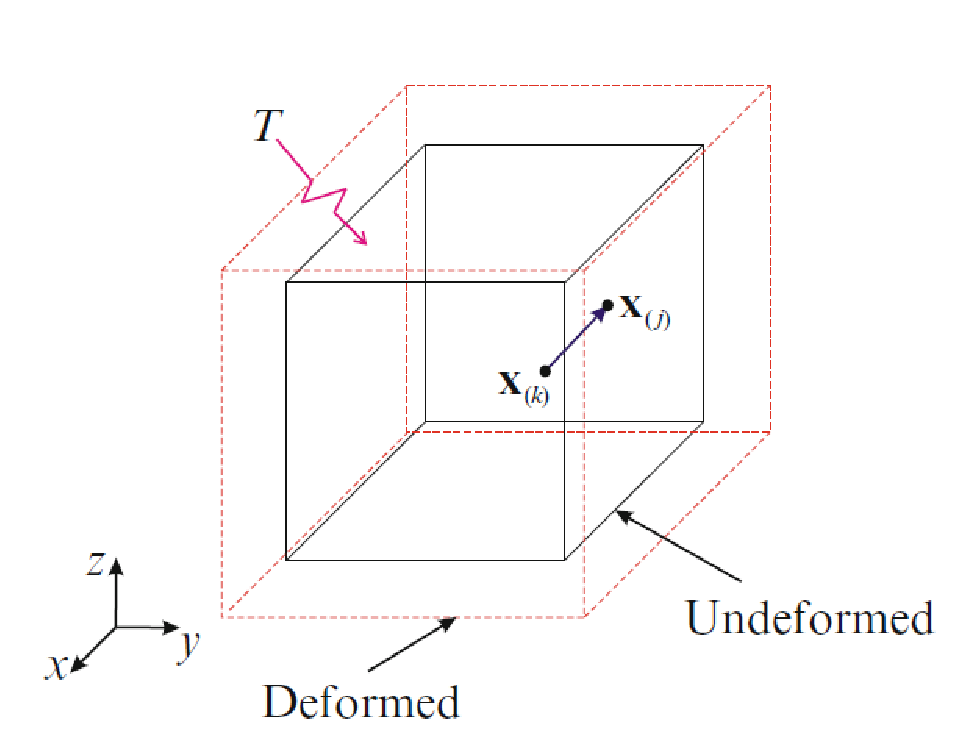
\includegraphics[width=0.5\linewidth]{E:/Thesis-Master/chap/image/pdm_isotropic_expansion}

  \caption{\label{pdm_isotropic_expansion}
           各向均匀膨胀下的三维物体。图片取自\mycite{Madenci}{2014}。
          }
\end{figure}

在各向均匀膨胀下,应变张量为

\begin{eqnarray}
  \epsilon_{xx(k)} =  \epsilon_{yy(k)} = \epsilon_{zz(k)} = \zeta\\
  \epsilon_{xy(k)} =  \epsilon_{xz(k)} = \epsilon_{yz(k)} = 0
\end{eqnarray}

则经典连续介质力学中的应变能量密度 $W_{(k)}$ 和 膨胀度$\theta_{(k)}$ 可显式算得为

\begin{equation}
W_{(k)} = \frac{9}{2}\kappa\zeta^2\\
\label{eq:33}
\end{equation}
\begin{equation}
\theta_{(k)} = \epsilon_{xx(k)}+\epsilon_{yy(k)}+\epsilon_{zz(k)} = 3\zeta.
\label{eq:34}
\end{equation}

并且形变后的相对位置可用未形变空间的相对位置表示为

\begin{equation}
|\mb{y}_{(j)} - \mb{y}_{(k)}| = (1+\zeta)|\mb{x}_{(j)} - \mb{x}_{(k)}|.
\label{eq:35}
\end{equation}

定义 $\bm{\xi} = \mb{x}_{(j)} - \mb{x}_{(k)}$, $\xi = |\bm{\xi}|$。
最终,$W_{(k)}$ 和 $\theta_{(k)}$ 的计算需要在半径为 $\delta$ 的圆球内进行积分:

\begin{equation}
\begin{aligned}
W_{(k)} =& a\theta_{(k)}^2
           +b\sum_{j=1}^{N}\omega_{(k)(j)}(s_{(k)(j)}|\mb{x}_{(j)}-\mb{x}_{(k)}|V_{(j)})\cdot(s_{(k)(j)}|\mb{x}_{(j)}-\mb{x}_{(k)}|V_{(j)})\\
        =& a\theta_{(k)}^2
           +b\int_0^\delta\int_0^{2\pi}\int_0^{\pi}\frac{\delta}{\xi}\left[(1+\zeta)\xi-\xi\right]^2\xi^2\sin(\phi)d\phi d\theta d\xi\\
        =& 9a\zeta^2+\pi b\delta^5\zeta^2
\end{aligned}
\label{eq:36}
\end{equation}
和
\begin{equation}
\begin{aligned}
\theta_{(k)} =& d\sum_{j=1}^{N}\omega_{(k)(j)}s_{(k)(j)}\frac{\mb{y}_{(j)} - \mb{y}_{(k)}}{|\mb{y}_{(j)} - \mb{y}_{(k)}|}\cdot(\mb{x}_{(j)}-\mb{x}_{(k)})V_{(j)}\\
        =& d\int_0^\delta\int_0^{2\pi}\int_0^{\pi}\frac{\delta}{\xi}\left[(1+\zeta)\xi-\xi\right](\frac{\bm{\xi}}{\xi}\cdot\frac{\bm{\xi}}{\xi})\xi^2\sin(\phi)d\phi d\theta d\xi\\
        =& \frac{4\pi d\delta^4}{3}\zeta,
\end{aligned}
\label{eq:37}
\end{equation}

其中$(\xi,\theta,\phi)$ 为球坐标。将方程 \ref{eq:36},\ref{eq:37}同方程\ref{eq:33},\ref{eq:34}进行对比,则可以得到两个重要的关系式:

\begin{equation}
9a + \pi b\delta^5 = \frac{9}{2}\kappa
\label{eq:38}
\end{equation}
\begin{equation}
d = \frac{9}{4\pi\delta^4}.
\label{eq:39}
\end{equation}

\noindent{\textbf{Case 2: 简单剪切}}

图\ref{pdm_simple_shear}所示为简单剪切形变下的三维物体。
\begin{figure}[htbp!]
  \centering
  \captionsetup{justification=centering}
  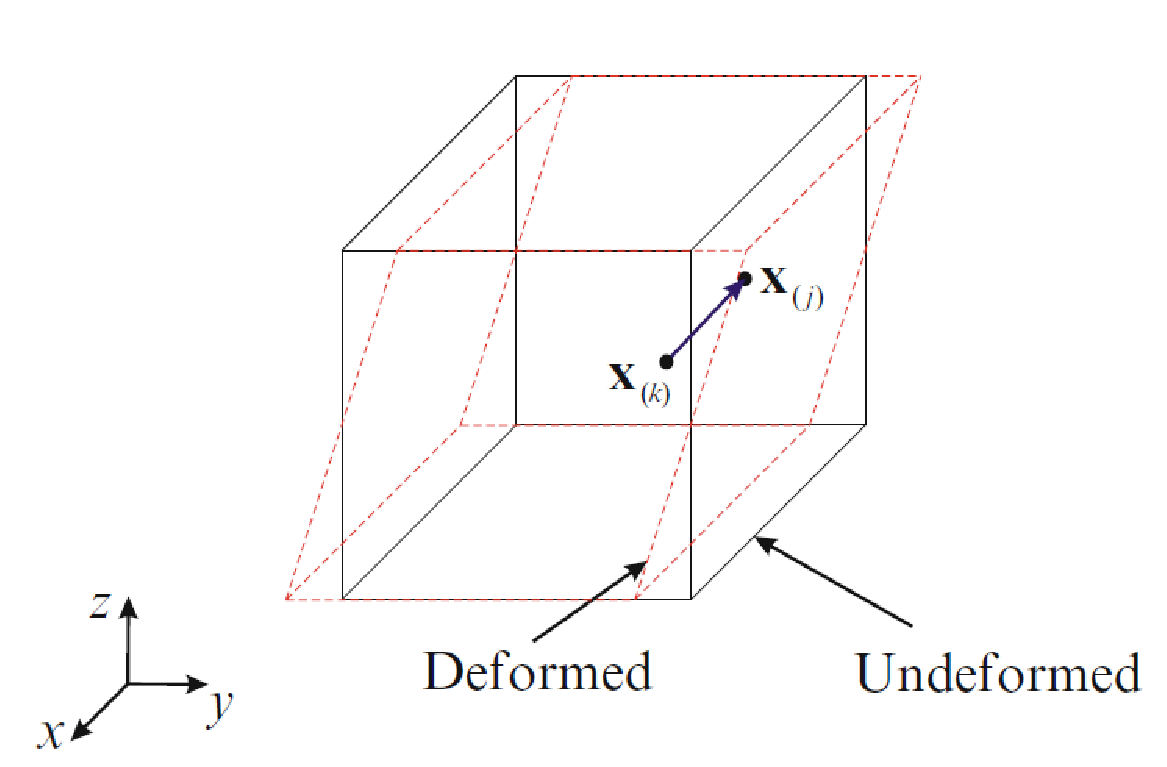
\includegraphics[width=0.5\linewidth]{E:/Thesis-Master/chap/image/pdm_simple_shear}

  \caption{\label{pdm_simple_shear}
           简单剪切形变下的三维物体。图片取自\mycite{Madenci}{2014}。
          }
\end{figure}

在这种情形下,有类比关系:
\begin{equation}
\gamma_{xy(k)} = \zeta
\label{eq:40}
\end{equation}
\begin{equation}
\sigma_{xx(k)} = \sigma_{yy(k)} = \sigma_{zz(k)} = \gamma_{xz(k)} =\gamma_{yz(k)} = 0
\label{eq:41}
\end{equation}
及
\begin{equation}
|\mb{y}_{(j)} - \mb{y}_{(k)}| = (1+\frac{\zeta\sin(2\phi)\sin(\theta)}{2})|\mb{x}_{(j)} - \mb{x}_{(k)}|.
\label{eq:42}
\end{equation}

连续介质力学下的$W_{(k)}$ 和 $\theta_{(k)}$则可以直接写为

\begin{equation}
W_{(k)} = \frac{1}{2}\mu\zeta^2\\
\label{eq:43}
\end{equation}
\begin{equation}
\theta_{(k)} = 0.
\label{eq:44}
\end{equation}

近场动力学下的$W_{(k)}$的值仍然需要通过半径为 $\delta$ 的圆球内进行积分来计算。即
\begin{equation}
\begin{aligned}
W_{(k)} =& b\sum_{j=1}^{N}\omega_{(k)(j)}(s_{(k)(j)}|\mb{x}_{(j)}-\mb{x}_{(k)}|V_{(j)})\cdot(s_{(k)(j)}|\mb{x}_{(j)}-\mb{x}_{(k)}|V_{(j)})\\
        =& b\int_0^\delta\int_0^{2\pi}\int_0^{\pi}\frac{\delta}{\xi}\left[(1+\frac{\zeta\sin(2\phi)\sin(\theta)}{2})\xi-\xi\right]^2\xi^2\sin(\phi)d\phi d\theta d\xi\\
        =& \frac{b\pi\delta^5\zeta^2}{15}.
\end{aligned}
\label{eq:45}
\end{equation}

比较 \ref{eq:43} 和 \ref{eq:45} 获得:
\begin{equation}
b = \frac{15\mu}{2\pi\delta^5}.
\label{eq:46}
\end{equation}

将方程 \ref{eq:46} 代入 \ref{eq:38} 则可以获得 $a$ 的具体形式:
\begin{equation}
a = \frac{1}{2}(\kappa - \frac{5\mu}{3}).
\label{eq:47}
\end{equation}

到此为止,三个动力学参数($a, b, d$)已经全部确定。

\subsubsection{最终模型}

本章节已经推导了从经典连续介质力学到近场动力学理论,各向同性线性材料的本构模型的整个演变过程。为免读者混淆以及方便后续章节引用,在此我们做简要总结。在 ordinary state based 模型下,力密度的计算通过如下方式计算:

\begin{equation}
\tkj = \frac{1}{2}A\frac{\bfyj - \bfyk}{|\bfyj - \bfyk|}
\end{equation}
其中
\begin{equation}
A = 4\wkj\left\{ad\frac{\bfyj-\bfyk}{|\bfyj-\bfyk|}\cdot\frac{\bfxj-\bfxk}{|\bfxj-\bfxk|}\thetak
   +b\left(|\bfyj - \bfyk| - |\bfxj - \bfxk|\right) \right\}
\end{equation}
\begin{equation}
\thetak = d\sum_{j=1}^{N}\wkj\skj\frac{\bfyj - \bfyk}{|\bfyj - \bfyk|}\cdot(\bfxj-\bfxk)V_{(j)}
\end{equation}
\begin{equation}
a = \frac{1}{2}(\kappa - \frac{5\mu}{3})
\end{equation}
\begin{equation}
b = \frac{15\mu}{2\pi\delta^5}
\end{equation}
\begin{equation}
d = \frac{9}{4\pi\delta^4}
\end{equation}